\section{Background}
\label{sec:background}
\subsection{Variational inference}
\label{subsec:variational}

Let $\mbx$ be a set of observations, $\mbz$ be latent variables, and
$\mblambda$ be the free parameters of a variational distribution
$q(\mbz; \mblambda)$. We aim to find the best approximation of the
posterior $p(\mbz\g \mbx)$ using the variational distribution
$q(\mbz; \mblambda)$, where the quality of the approximation is
measured by KL divergence. This is equivalent to maximizing the
quantity
\begin{equation*}
\mathcal{L}\left(\mblambda\right)
 = \mathbb{E}_{q(\mbz;\mblambda)}[\log p(\mbx,\mbz)]
 - \mathbb{E}_{q(\mbz;\mblambda)}[\log
 q(\mbz;\mblambda)].
\end{equation*}
$\mathcal{L}(\mblambda)$ is the \emph{\gls{ELBO}}, or the variational free
energy~\citep{wainwright2008graphical}.
\if0
\begin{equation*}
\mathcal{L}\left(\mblambda\right)
 = \underbrace{\mathbb{E}_{q(\mbz;\mblambda)}[\log p(\mbx,\mbz)]}_{\text{energy}} \underbrace{- \mathbb{E}_{q(\mbz;\mblambda)}[\log
 q(\mbz;\mblambda)]}_{\text{entropy}}.
\end{equation*}
$\mathcal{L}(\mblambda)$ is the \emph{\gls{ELBO}}, or the variational free
energy~\citep{wainwright2008graphical}.
% Interpreting the ELBO
We say the first and second terms of the \gls{ELBO} are the energy and
entropy respectively: the energy rewards variational distributions
which explain the observations (and prior), and the entropy rewards
distributions that spread out their mass.  When optimizing, these
terms are at odds.
\fi
%
For simpler computation, a standard choice of the variational family
is a \emph{mean-field approximation}
\begin{equation*}
  q(\mbz;\mblambda) = \prod_{i=1}^{d} q_{i}(\mbz_{i};\mblambda_i),
\end{equation*}
where $\mbz=(\mb\mbz_1,\ldots,\mb\mbz_d)$. Note this is a strong independence
assumption.  More sophisticated approaches, known as \emph{structured
  variational inference}~\citep{saul1995exploiting}, attempt to restore
some of the dependencies among the latent variables.

In this work, we restore dependencies using copulas. Structured
\gls{VI} is typically tailored to individual models and is difficult
to work with mathematically. Copulas learn general posterior
dependencies during inference, and they do not require the
investigator to know such structure in advance. Further, copulas can
augment a structured factorization in order to introduce
dependencies that were not considered before; thus it generalizes
the procedure. We next review copulas.

\subsection{Copulas}
\label{subsec:copulas}

We will augment the mean-field distribution with a \emph{copula}. We
consider the variational family
\begin{equation*}
  q(\mbz) = \left[\prod_{i=1}^d q(\mbz_i)\right] c(Q(\mbz_1),\ldots,Q(\mbz_d)).
\end{equation*}
Here $Q(\mbz_i)$ is the marginal cumulative distribution function (CDF)
of the random variable $\mbz_i$, and $c$ is a joint distribution of
$[0,1]$ random variables.\footnote{We overload the notation for the
  marginal CDF $Q$ to depend on the names of the argument, though we
  occasionally use $Q_i(\mbz_i)$ when more clarity is needed. This is
  analogous to the standard convention of overloading the probability
  density function $q(\cdot)$.}  The distribution $c$ is called
a copula of $\mbz$: it is a joint multivariate density of
$Q(\mbz_1),\ldots,Q(\mbz_d)$ with uniform marginal
distributions~\citep{sklar1959fonstions}.  For any distribution, a
factorization into a product of marginal densities and a copula always
exists and integrates to one~\citep{nelsen2006introduction}.

Intuitively, the copula captures the information about the
multivariate random variable after eliminating the marginal
information, i.e., by applying the probability integral transform on
each variable. The copula captures only and all of the dependencies
among the $\mbz_i$'s. Recall that, for all random variables, $Q(\mbz_i)$ is
uniform distributed. Thus the marginals of the copula give no
information.

For example, the bivariate Gaussian copula is defined as
\begin{equation*}
  c(\mbu_1, \mbu_2; \rho)= \Phi_\rho(\Phi^{-1}(\mbu_1),
  \Phi^{-1}(\mbu_2)).
\end{equation*}
If $\mbu_1,\mbu_2$ are independent uniform distributed, the inverse CDF
$\Phi^{-1}$ of the standard normal transforms $(\mbu_1,\mbu_2)$ to independent
normals. The CDF $\Phi_{\rho}$ of the bivariate Gaussian
distribution, with mean zero and Pearson correlation $\rho$, squashes the
transformed values back to the unit square.
Thus the Gaussian copula directly correlates $\mbu_1$ and $\mbu_2$
with the Pearson correlation parameter $\rho$.

\subsubsection{Vine copulas}
\label{subsubsec:vine}

It is difficult to specify a copula.  We must find a family of
distributions that is easy to compute with and able to express a broad
range of dependencies.  Much work focuses on two-dimensional copulas,
such as the Student-$t$, Clayton, Gumbel, Frank, and Joe copulas
\citep{nelsen2006introduction}. However, their multivariate extensions
do not flexibly model dependencies in higher
dimensions~\citep{genest2009editorial}. Rather, a successful approach
in recent literature has been by combining sets of conditional
bivariate copulas; the resulting joint is called a \emph{vine}~\citep{joe1996families,kurowicka2006uncertainty}.

A vine $\mathcal{V}$ factorizes a copula density $c(\mbu_1,\ldots,\mbu_d)$
into a product of conditional bivariate copulas, also called pair
copulas.  This makes it easy to specify a high-dimensional copula.
One need only express the dependence for each pair of random variables
conditioned on a subset of the others.

\begin{figure}[t]
\centering
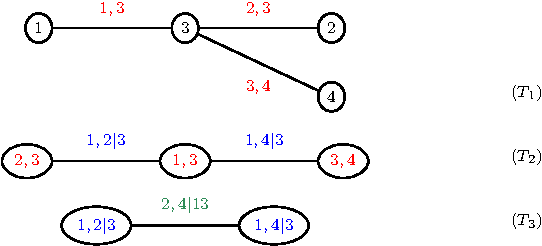
\includegraphics[width=0.75\textwidth]{img/vine_copula.pdf}
\caption{Example of a vine $\mathcal{V}$ which factorizes a copula density of
four random variables $c(\mbu_1,\mbu_2,\mbu_3,\mbu_4)$ into a product
of 6 pair
copulas. Edges in the tree $T_j$ are the nodes of the lower level tree
$T_{j+1}$, and each edge determines a bivariate copula which is conditioned on
all random variables that its two connected nodes share.}
\label{fig:vine_copula}
\end{figure}

\myfig{vine_copula} is an example of a vine which factorizes a
4-dimensional copula into the product of 6 pair copulas. The first
tree $T_1$ has nodes $1,2,3,4$ representing the random variables
$\mbu_1,\mbu_2,\mbu_3,\mbu_4$ respectively. An edge corresponds
to a pair copula, e.g., $1,4$ symbolizes $c(\mbu_1,\mbu_4)$. Edges in
$T_1$ collapse into nodes in the next tree $T_2$, and edges in $T_2$
correspond to conditional bivariate copulas, e.g., $1,2|3$ symbolizes
$c(\mbu_1,\mbu_2|\mbu_3)$. This proceeds to the last
nested tree $T_3$, where $2,4|13$ symbolizes
$c(\mbu_2,\mbu_4|\mbu_1,\mbu_3)$. The vine structure specifies a
complete factorization of the multivariate copula, and each pair
copula can be of a different family with its own set of parameters:
\begin{align*}
c(\mbu_1,\mbu_2,\mbu_3,\mbu_4) =
\Big[c(\mbu_1,\mbu_3)c(\mbu_2,\mbu_3)c(\mbu_3,\mbu_4)\Big]
\Big[c(\mbu_1,\mbu_2|\mbu_3)c(\mbu_1,\mbu_4|\mbu_3)\Big]
\Big[c(\mbu_2,\mbu_4|\mbu_1,\mbu_3)\Big].
\end{align*}
%
Formally, a vine is a nested set of trees
$\mathcal{V} = \{T_1,\ldots, T_{d-1}\}$ with the following
properties:
%\footnote{What we define as vines are also known as \emph{regular
%vines} in the literature. They are a generalization of other types of
%pair copula constructions such as the canonical vines and drawable
%vines~\citep{dissmann2012selecting}.}
\begin{enumerate}
\item Tree $T_j=\{N_j,E_j\}$ has $d+1-j$ nodes and $d-j$ edges.
\item Edges in the $j^{th}$ tree $E_j$ are the nodes in the $(j+1)^{th}$ tree $N_{j+1}$.
\item %\emph{Proximity condition}:
Two nodes in tree $T_{j+1}$ are joined by an edge only if the corresponding edges in tree $T_{j}$ share a node.
\end{enumerate}
%
Each edge $e$ in the nested set of trees $\{T_1,\ldots,T_{d-1}\}$
specifies a different pair copula, and the product of all edges
comprise of a factorization of the copula density. Since there are a
total of $d(d-1)/2$ edges, $\mathcal{V}$ factorizes
$c(\mbu_1,\ldots,\mbu_d)$ as the product of $d(d-1)/2$ pair copulas.

Each edge
$e(i,k) \in T_j$ has a
\emph{conditioning set} $D(e)$, which is a set of variable indices
$1,\ldots,d$. We define
$c_{ik|D(e)}$ to be the bivariate copula density for $\mbu_i$ and
$\mbu_k$ given its conditioning set:
\begin{equation}
c_{ik|D(e)} = c\Big( Q(\mbu_i|\mbu_j : j \in D(e)), Q(\mbu_i|\mbu_j :
j \in D(e)) \Big| \mb\mbu_j : j\in D(e)\Big).
\label{eq:defcjk}
\end{equation}
Both the copula and the CDF's in its arguments are conditional
on $D(e)$. A vine specifies a factorization of the
copula, which is a product over all edges in the $d-1$ levels:
\begin{equation}
  c(\mbu_1,\ldots,\mbu_d; \mbeta) = \prod_{j=1}^{d-1}\prod_{e(i,k)\in E_j} c_{ik|D(e)}.
\label{eq:vinedecomp}
\end{equation}
%
% [todo] below, we are suddenly discussing the parameters to these
% copulas.  they don't appear above.  i think you need to introduce
% this idea more slowly, perhaps introducing parameters above.  it is
% crucial for what follows (i.e., our work). --dmb
%
We highlight that $c$ depends on $\mbeta$, the set of all parameters to
the pair copulas.  The vine construction provides us with the
flexibility to model dependencies in high dimensions using a
decomposition of pair copulas which are easier to estimate. As we
shall see,
the construction also leads to efficient stochastic gradients by
taking individual (and thus easy) gradients on each pair copula.

%%% Local Variables:
%%% mode: latex
%%% TeX-master: "nips2015"
%%% End:
